\subsubsection{\textit{Khảo sát cấu hình của máy và hệ thống bộ nhớ của máy đang sử dụng (Bộ nhớ trong: ROM, RAM, Cache System; Bộ nhớ ngoài: ổ đĩa cứng, CD, Thiết bị vào ra)}}

\noindent\textbf{\large Phần mềm khảo sát:} 
\begin{itemize}
    \item Sử dụng phần mềm CPU-Z 64-bit Ver. 2.15
    \item Sử dụng các chương trình quản lí đĩa và thiết bị trên máy tính (Disk Management và Device Manager)
\end{itemize}

\vspace{0.5cm}

% --- CPU ---
\noindent\textbf{\large CPU:} (Thông số chi tiết thể hiện ở Hình \ref{fig:cpu-z-cpu})

\begin{itemize}
    \item \textbf{Tên CPU:} Intel Core i3-10110U
    \item \textbf{Kiến trúc:} Comet Lake-U/Y
    \item \textbf{Tiến trình sản xuất:} 14nm
    \item \textbf{TDP tối đa:} 15W (rất tiết kiệm điện, phù hợp cho laptop)
    \item \textbf{Socket:} 1528 FCBGA (dạng hàn chết lên mainboard, phổ biến ở laptop)
    \item \textbf{Số nhân - Số luồng:} 2 nhân, 4 luồng
    \item \textbf{Xung nhịp cơ bản:} 2.10 GHz (thể hiện ở dòng "Specification")
    \item \textbf{Xung nhịp hiện tại:} Khoảng 900 MHz
    \item \textbf{Bus Speed:} 100.35 MHz
    \item \textbf{Tập lệnh hỗ trợ:} MMX, SSE (và các biến thể), AVX, AVX2, FMA3,...
\end{itemize}

\begin{center}
    \fbox{\parbox{0.9\textwidth}{
        \centering
        \large Đây là một CPU tiết kiệm điện, phổ biến trên các laptop mỏng nhẹ, hiệu năng vừa đủ cho các tác vụ văn phòng, học tập, hoặc giải trí nhẹ nhàng.
    }}
\end{center}

\begin{figure}[H]
    \centering
    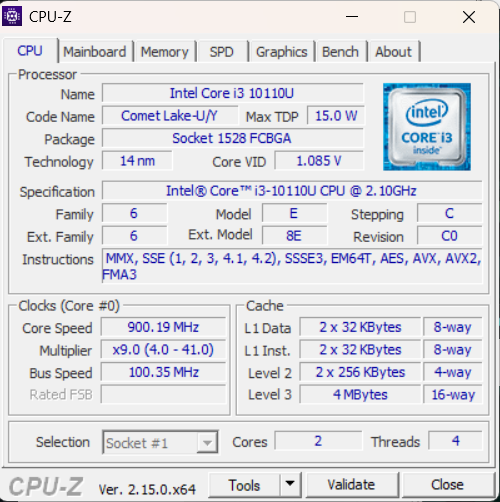
\includegraphics[width=0.75\textwidth]{Images/Stats/CPU.png}
    \caption{Giao diện phần mềm CPU-Z - Tab CPU}
    \label{fig:cpu-z-cpu}
\end{figure}

% --- Cache ---
\noindent\textbf{\large Cache:} (Thông số chi tiết thể hiện ở Hình \ref{fig:cpu-z-cache})

\begin{itemize}
    \item \textbf{L1 Cache (Level 1 Cache):}
    \begin{itemize}
        \item \textbf{Data:} 2 × 32 KB
        \item \textbf{Instruction:} 2 × 32 KB
        \item \textbf{Tổ chức:} 8-way associative (8 đường liên kết)
        \item \textit{Ghi chú:} Đây là bộ nhớ cache nhanh nhất và nhỏ nhất, chia riêng biệt cho dữ liệu và lệnh. Mỗi nhân có cache riêng.
    \end{itemize}
    
    \item \textbf{L2 Cache (Level 2 Cache):}
    \begin{itemize}
        \item \textbf{Dung lượng:} 2 × 256 KB
        \item \textbf{Tổ chức:} 4-way associative
        \item \textit{Ghi chú:} Mỗi nhân có 256 KB cache L2 riêng biệt, trung gian giữa L1 và L3.
    \end{itemize}
    
    \item \textbf{L3 Cache (Level 3 Cache):}
    \begin{itemize}
        \item \textbf{Dung lượng:} 4 MB (chia sẻ giữa các nhân)
        \item \textbf{Tổ chức:} 16-way associative
        \item \textit{Ghi chú:} Đây là cache lớn nhất và được chia sẻ chung cho tất cả các nhân CPU, giúp giảm độ trễ khi trao đổi dữ liệu giữa các nhân.
    \end{itemize}
\end{itemize}

\begin{center}
    \fbox{\parbox{0.9\textwidth}{
        \centering
        \large Cache cấp thấp hơn (L1) thì nhỏ nhưng cực nhanh, trong khi cấp cao hơn (L3) thì lớn hơn nhưng tốc độ chậm hơn. Cấu trúc nhiều cấp như vậy giúp tối ưu tốc độ truy xuất bộ nhớ của CPU.
    }}
\end{center}

\begin{figure}[H]
    \centering
    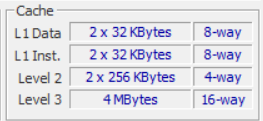
\includegraphics[width=0.5\textwidth]{Images/Stats/Cache.png}
    \caption{Giao diện phần mềm CPU-Z - Bộ nhớ Cache}
    \label{fig:cpu-z-cache}
\end{figure}

% --- RAM ---
\noindent\textbf{\large RAM:} (Thông số chi tiết thể hiện ở Hình \ref{fig:cpu-z-memory})

\begin{itemize}
    \item \textbf{Loại RAM:} DDR4
    \item \textbf{Dung lượng:} 8 GB
    \item \textbf{Số kênh (Channel):} Dual (2 kênh)
    \item \textbf{Tần số thực tế (DRAM Frequency):} 665.5 MHz
    \item \textbf{Tỉ lệ FSB:DRAM:} 3:20
    \item \textbf{Độ trễ CAS (CL):} 10.0 clocks
    \item \textbf{RAS to CAS Delay (tRCD):} 10 clocks
    \item \textbf{RAS Precharge (tRP):} 10 clocks
    \item \textbf{Cycle Time (tRAS):} 28 clocks
    \item \textbf{Row Refresh Cycle Time (tRFC):} 234 clocks
    \item \textbf{Command Rate (CR):} 1T
\end{itemize}

\begin{center}
    \fbox{\parbox{0.9\textwidth}{
        \centering
        \large RAM của hệ thống này có cấu hình cân bằng, đáp ứng tốt nhu cầu phổ thông, đồng thời nhờ Dual Channel mà hiệu suất cũng khá ổn định và mượt mà trong các tác vụ đa nhiệm.
    }}
\end{center}

\begin{figure}[H]
    \centering
    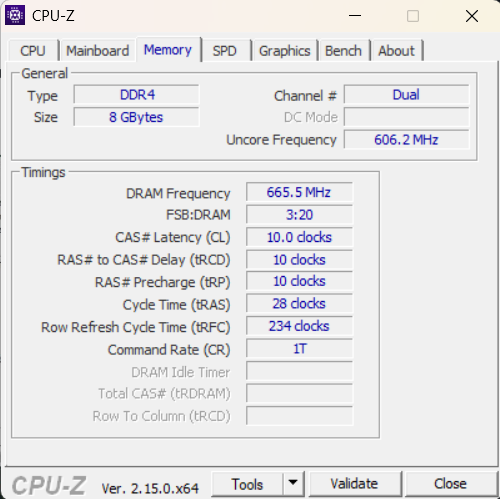
\includegraphics[width=0.5\textwidth]{Images/Stats/Memory.png}
    \caption{Giao diện phần mềm CPU-Z - Bộ nhớ}
    \label{fig:cpu-z-memory}
\end{figure}

% --- Bộ nhớ ngoài ---
\noindent\textbf{\large Bộ nhớ ngoài:} (Thông số chi tiết thể hiện ở Hình \ref{fig:cpu-z-disk})

\begin{itemize}
    \item \textbf{Ổ cứng:} 1 ổ cứng vật lý (Disk 0)
    \item \textbf{Dung lượng tổng:} 238.46 GB
    \item \textbf{Cấu trúc phân vùng:}
    \begin{itemize}
        \item \textbf{OS (C:)} 119.60 GB (NTFS)
        \begin{itemize}
            \item Phân vùng chứa hệ điều hành Windows.
            \item Còn trống: 33.73 GB (khoảng 28\% dung lượng).
        \end{itemize}
        \item \textbf{Data (D:)} 117.19 GB (NTFS)
        \begin{itemize}
            \item Phân vùng lưu trữ dữ liệu cá nhân.
            \item Còn trống: 110.64 GB (khoảng 94\% dung lượng).
        \end{itemize}
        \item \textbf{Phân vùng hệ thống và khôi phục:}
        \begin{itemize}
            \item 260 MB (EFI System Partition) -- phân vùng khởi động.
            \item 1.22 GB (Recovery Partition) -- phân vùng phục hồi hệ thống.\\Dùng để khôi phục máy về trạng thái ban đầu (Factory Reset) như lúc mới mua.
            \item 200 MB (Recovery Partition) -- phân vùng phục hồi hệ thống.\\Dùng để sửa lỗi khởi động (Startup Repair), khôi phục hệ thống (System Restore), reset PC (Reset This PC), hoặc truy cập Command Prompt khi hệ điều hành gặp sự cố.
        \end{itemize}
    \end{itemize}
    \item \textbf{Hệ thống tập tin:} NTFS cho các phân vùng chính.
\end{itemize}

\begin{center}
    \fbox{\parbox{0.9\textwidth}{
        \centering
        \large Ổ đĩa đang được phân vùng hợp lý, tách riêng dữ liệu và hệ điều hành. Dung lượng dữ liệu còn trống nhiều, không có phân vùng lỗi, hệ thống đang vận hành ổn định.
    }}
\end{center}

\begin{figure}[H]
    \centering
    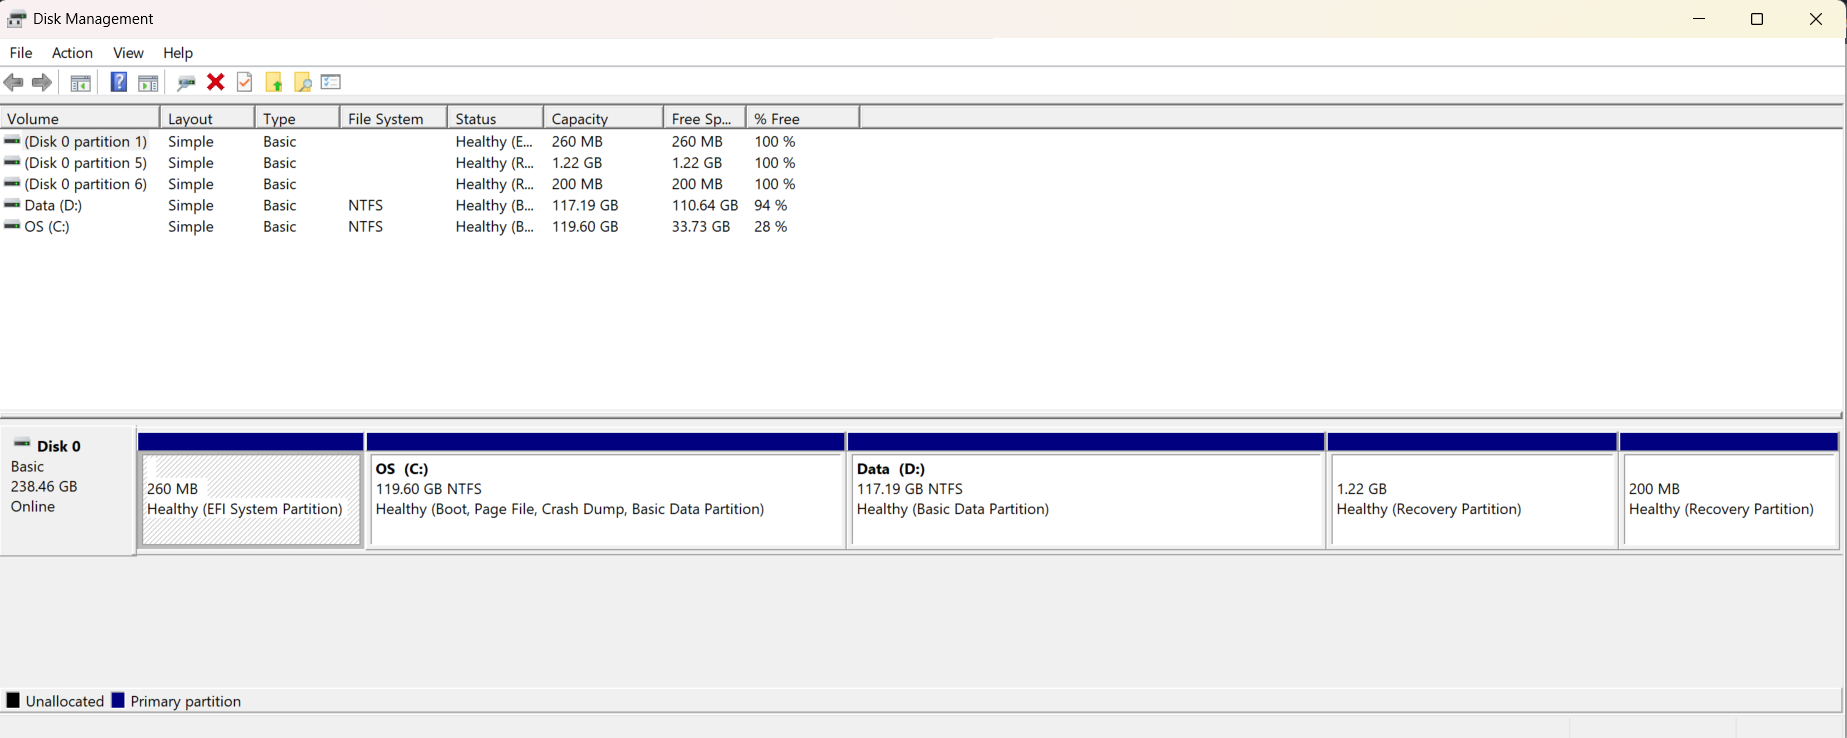
\includegraphics[width=0.9\textwidth]{Images/Stats/Disk.png}
    \caption{Giao diện chương trình Disk Management}
    \label{fig:cpu-z-disk}
\end{figure}

% --- Các thiết bị vào ra ---
\noindent\textbf{\large Các thiết bị vào ra:} (Thông số chi tiết thể hiện ở Hình \ref{fig:cpu-z-device})

\begin{itemize}
        \item \textbf{Thiết bị âm thanh (Audio inputs and outputs):} 
        \begin{itemize}
            \item \textbf{Microphone:} Realtek(R) Audio: microphone tích hợp.
            \item \textbf{Speakers:} Realtek(R) Audio: loa tích hợp laptop.
        \end{itemize}
        \item \textbf{Thiết bị nhập liệu giao tiếp người dùng (Human Interface Devices):} 
        \begin{itemize}
            \item \textbf{ASUS Precision Touchpad:} touchpad của laptop ASUS.
            \item \textbf{Nhiều thiết bị HID-compliant khác (chuột, bàn di, điều khiển hệ thống, v.v.):} các thiết bị phụ trợ nhập liệu như chuột rời, touchpad, bàn phím rời, các nút multimedia...
        \end{itemize}
        \item \textbf{Bàn phím (Keyboards):}
        \begin{itemize}
            \item \textbf{3 thiết bị HID Keyboard Device:} bàn phím laptop + bàn phím ảo + bàn phím rời.
            \item \textbf{PC/AT Enhanced PS/2 Keyboard (101/102-Key):} bàn phím vật lý mặc định gắn với mainboard qua cổng PS/2 hoặc emulated PS/2.
        \end{itemize}
        \item \textbf{Chuột và các thiết bị trỏ khác (Mice and other pointing devices):}
        \begin{itemize}
            \item \textbf{3 thiết bị HID-compliant mouse:} touchpad, chuột ngoài, hoặc thiết bị trỏ phụ (ví dụ: trackpoint, bút stylus...).
        \end{itemize}
    \end{itemize}

\begin{center}
    \fbox{\parbox{0.9\textwidth}{
        \centering
        \large Laptop đang sử dụng đa dạng và hiệu quả các thiết bị vào ra, từ đó mang lại trải nghiệm sử dụng tốt nhất cho người dùng.
    }}
\end{center}

\begin{figure}[H]
    \centering
    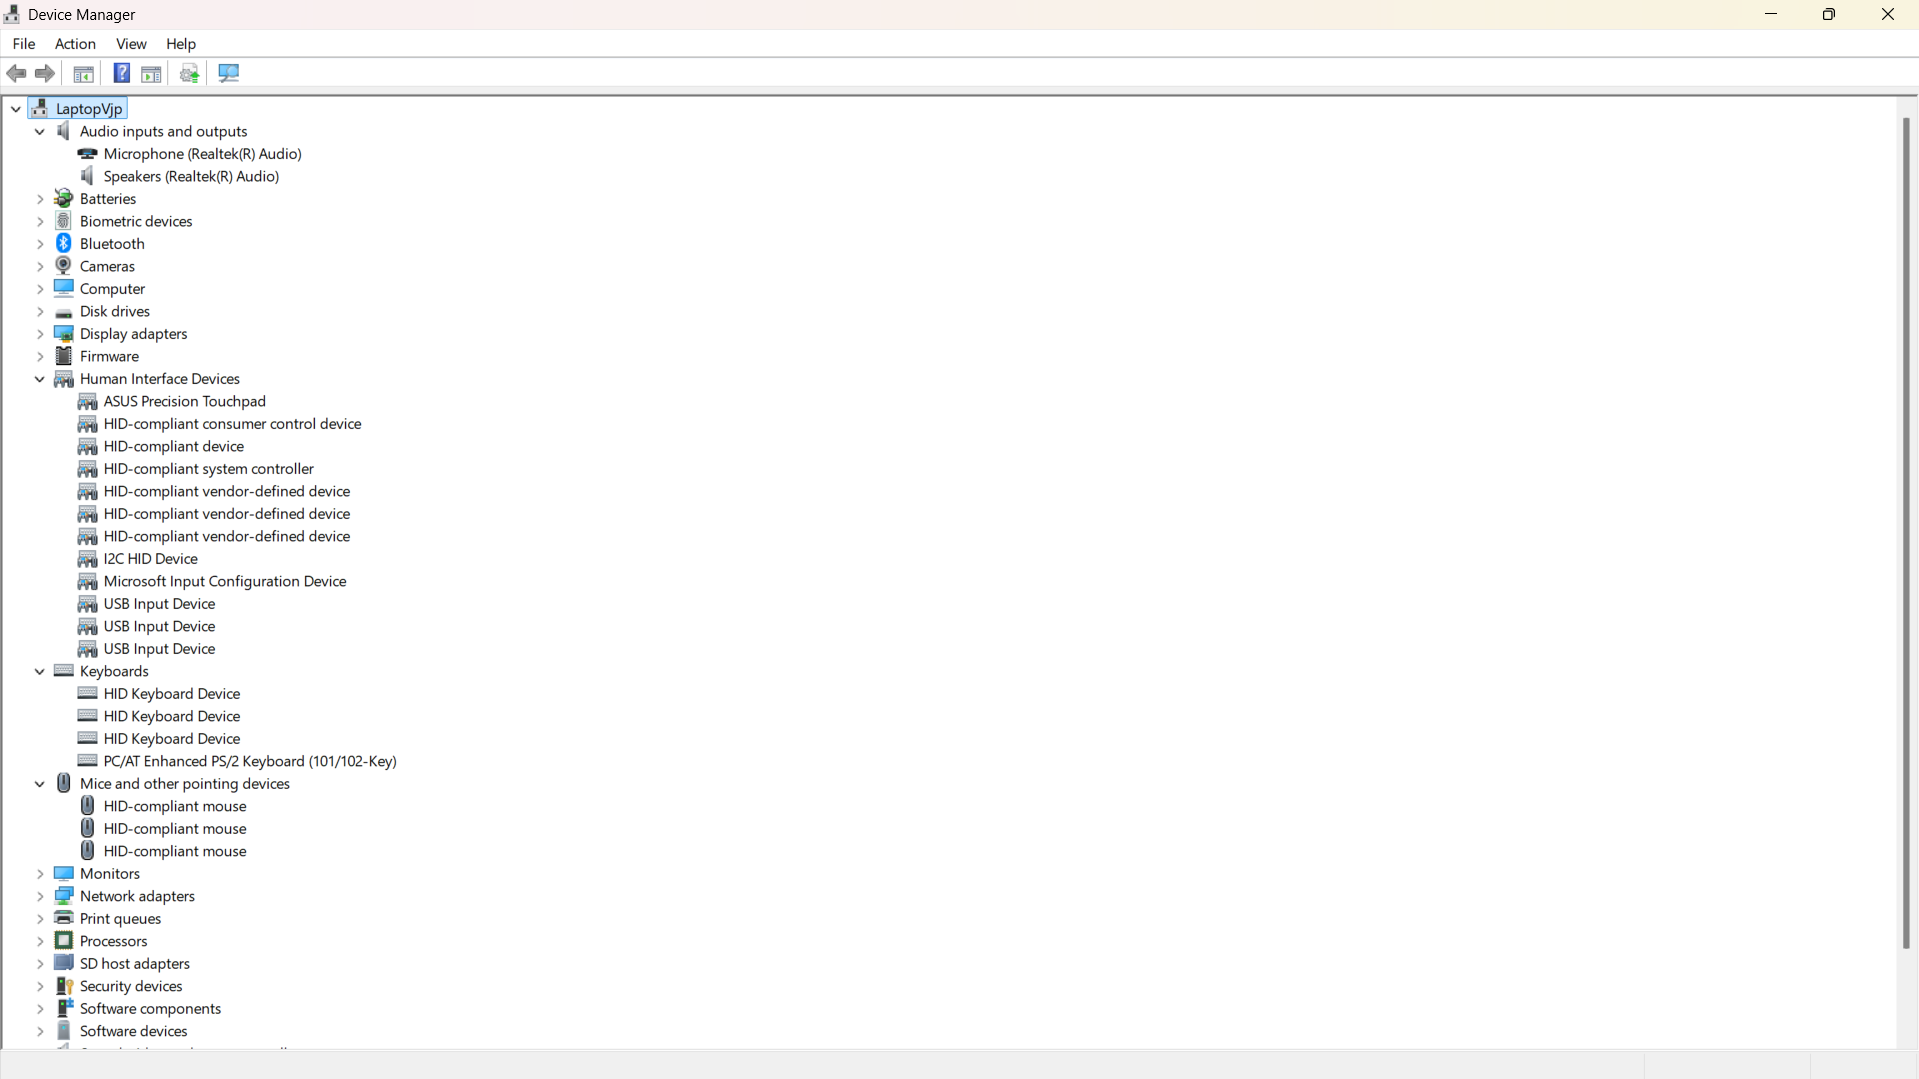
\includegraphics[width=1\textwidth]{Images/Stats/Device.png}
    \caption{Giao diện chương trình Device Manager}
    \label{fig:cpu-z-device}
\end{figure}